\chapter{VISUAL SOLUTIONS FOR DOI INTERPRETATION}
In this chapter we discuss the possible visual interpretations for DOI data. AOI is image-space counter part of DOI. Although plethora of visual solutions exist for AOI~\cite{Bla14}, three distinct properties of DOIs prohibit them to interpret DOI data. First, DOI data has volumes and multiple granularities. Second, DOI data deals with data attributes. Third, DOI data supports different range of analysis questions possible compared to AOI data. 

\section{Existing Visualizations for Eye-tracking Data}
\label{sec:ClassicVisualization}
In this section, we discuss existing visualization techniques for eye-tracking data. Specifically, we will focus on three basic visualization techniques: Heatmap, Scanpath, and Scarfplot. %Moreover, we will briefly discuss about three advanced techniques : AOI-river, Transition Matrices, and Directed graphs.

\subsection{Heatmap}
Heatmap visualization contains a 2D matrix where each cell is assigned a color. The color used in the cell represent value of the cell. Multiple color schemes exist to represent color to value. The most popular color scheme is the 'Rainbow' color scheme. In rainbow color scheme, 'red' represents maximum and 'violet' represents minimum. Many heatmap visualizations also use green or blue for minimum. However, rainbow color scheme lacks perceptual ordering, and not sensitive small value changes~\cite{borland2007rainbow}. Hence, visualization researchers consider rainbow color scheme as misleading. Many heatmaps use color scales such as gray-scale, heated-object, and linearized optimal scale~\cite{silva2007there}. Figure~\ref{fig:heatmapsExample} depicts an example of heatmaps with three different color schemes. 

\begin{figure}[htbp]
  \centering
  \includegraphics[width=\linewidth]{images/heatmapsExample.eps}
  \caption{Heatmap visualization with three different color schemes: (a) rainbow, (b) gray-scale, and (c) heated object.}
	\label{fig:heatmapsExample}
\end{figure}



\subsection{Scanpath}
A scanpath visualization depicts transitions among multiple entities over time. Scanpath visualization either show temporal information in a linear scale or discard temporal information. For example, we encode transitions among five entities $e_1 \rightarrow e_2\rightarrow e_3\rightarrow e_4\rightarrow e_5\}$ with scanpath visualization. Figure~\ref{fig:scanpathExample}(a) portray all transitions among entity to entity. Such techniques require a layout with minimal crossing among transitions. However, it produces a compact visualization. Again, in Figure~\ref{fig:scanpathExample}(b), all entities lie vertically and are connected with a horizontal line to show temporal information. For depicting a transition between $e_1$ and $e_2$, we place transition markers (e.g. a circle) along their horizontal lines. Then, we connect the markers with transition encoding (e.g. an arrow). The latter technique is more suitable for following transitions. However, it takes more space than the former version. 

\begin{figure}[htbp]
  \centering
  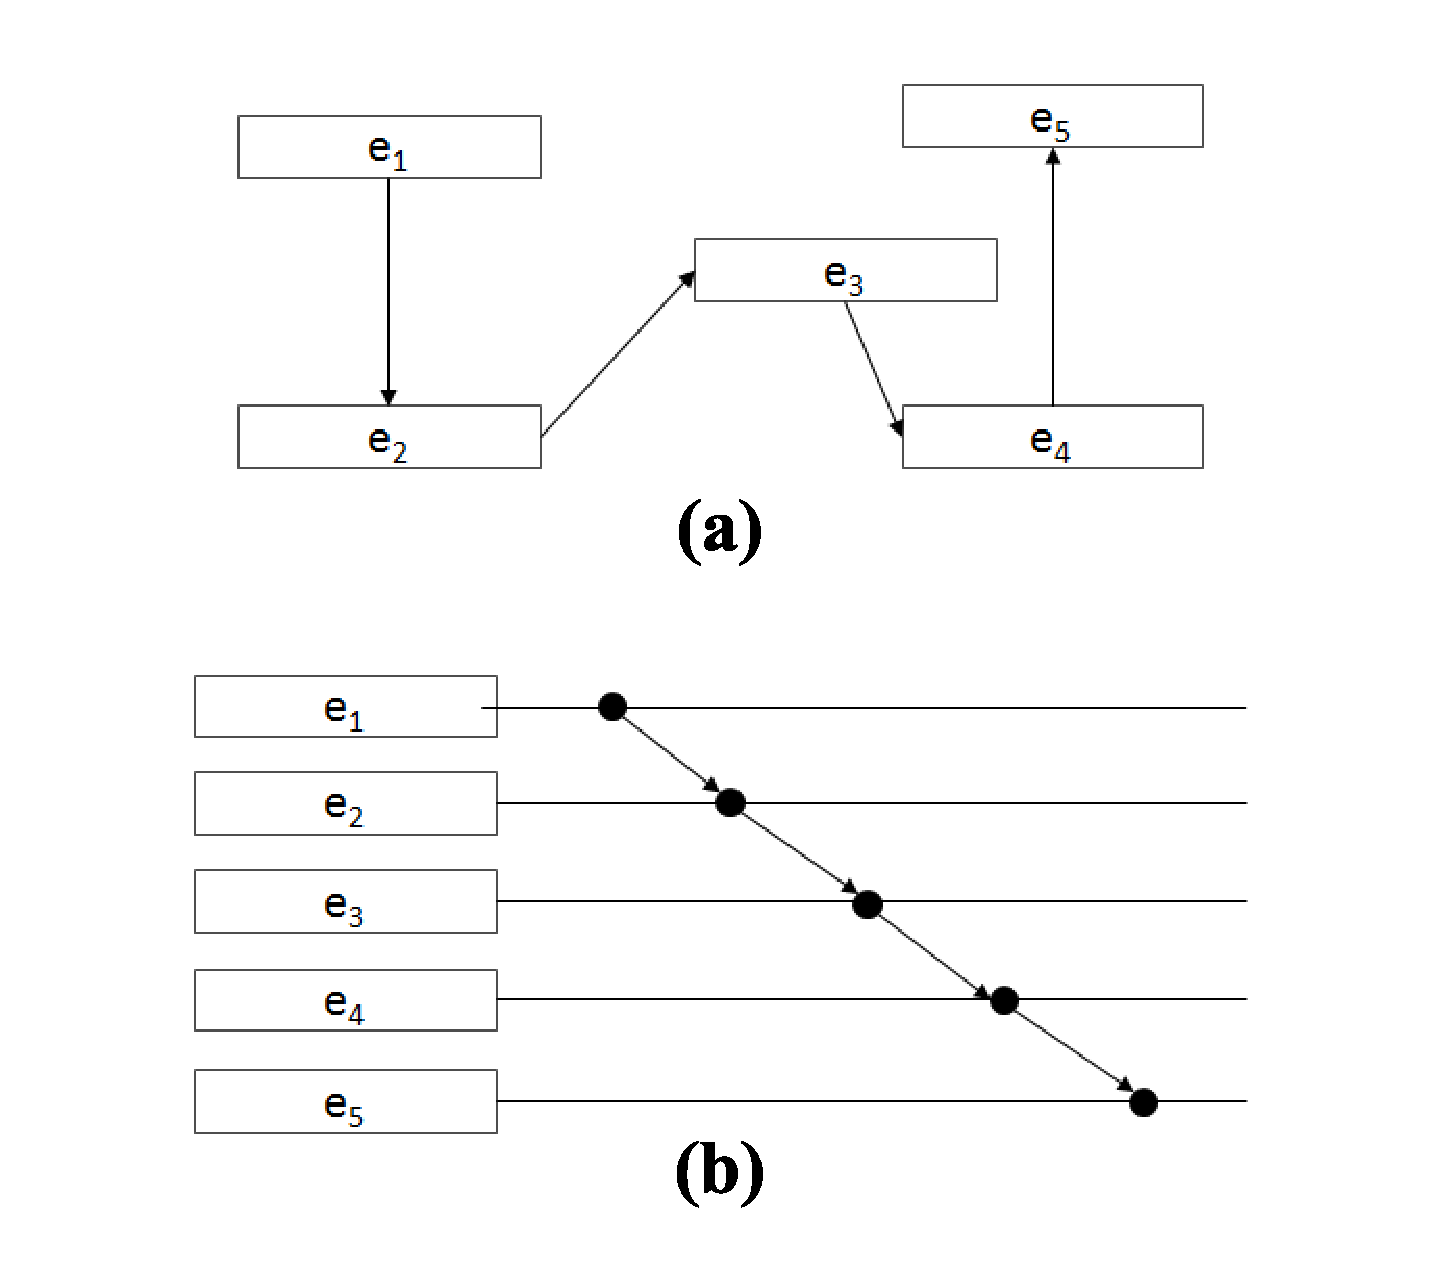
\includegraphics[width=\linewidth]{images/scanpathExample.eps}
  \caption{Scanpath visualization (a) without explicit temporal information, (b) with temporal transitions.}
	\label{fig:scanpathExample}
\end{figure}

\subsection{Scarfplot}
In a scarplot technique, visual entities are joined as multiple tapes known as scarflines~\cite{richardson2005looking}. The entities may have different width in tapes. The width usually represent data value (e.g. intensity). Figure~\ref{fig:scarfplotExample} demonstrate an example of transitions viewing pattern for two users. $User_1$ viewed entities $e_1, e_2, e_3, e_4,e_5$ and $User_2$ viewed $e_6, e_7$. Scarfplot technique is useful for finding pattern among multiple sets of data. 
\begin{figure}[htbp]
  \centering
  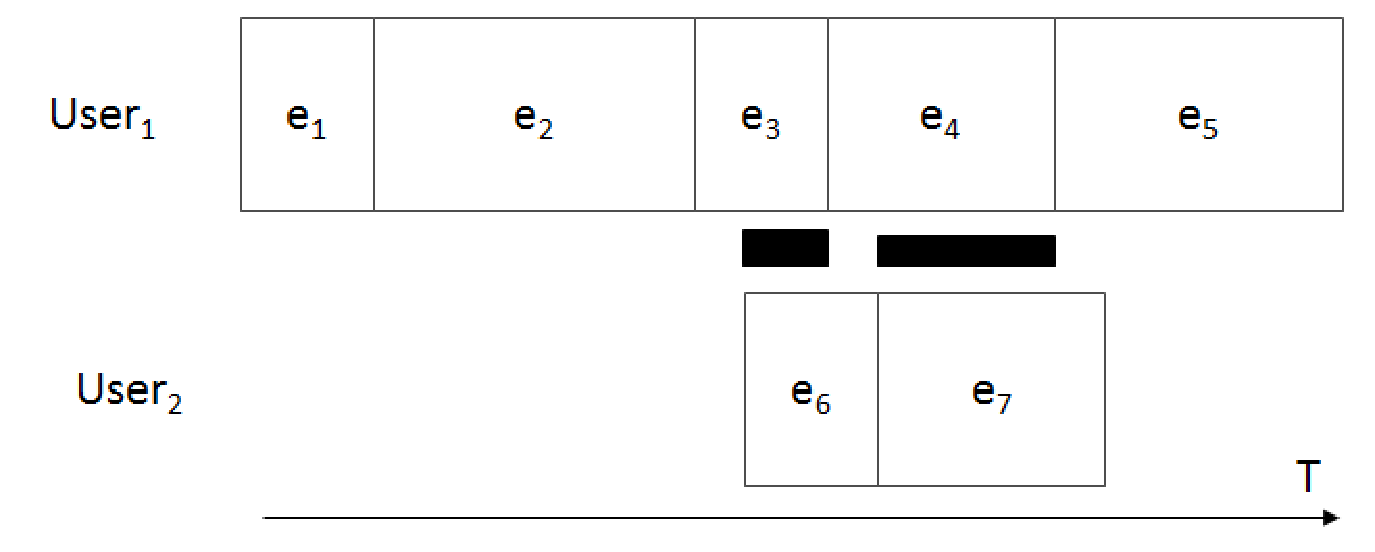
\includegraphics[width=\linewidth]{images/ScarfplotExample.eps}
  \caption{An example of Scarfplot visualization. }
	\label{fig:scarfplotExample}
\end{figure}

\section{Enhancing Visualization for DOI Data}
Visualization techniques discussed in Section~\ref{sec:ClassicVisualization} can interpret DOI data with several limitations. First, heatmap visualization dimension may exceed due to large data scale DOI data. The example depicted in Figure~\ref{fig:heatmapsExample} shows a 2D matrix of $5 \times 26$ dimensions. If we want to use heatmap for DOI data, then dimension may exceed $100 \times 100$. For example, a DOI data of time length 3 minute may produce a heatmap of $180 \times 75$ (i.e. 1 second per time cell and maximum 75 DOIs detected in 1 sec). Thus, we need filtration and sorting in such cases. Second, scanpath diagram have similar dimension related problem. However, with the increasing amount of DOIs will produce cluttering in transitions. Hence, the ordering DOI elements are vital in such cases. We can use clustering to solve this problem. Third, scarfplot are suitable for interpreting DOIs in a compact manner. However, labels are not clearly visible in a scarfplot. Thus, distinguishing DOI elements will be challenging. To solve this, we may use different textures and encoding for DOI data elements in scarflines. We discuss possible enhancements for DOI visualization below. 

\subsection{Handling Large Data Scale and Multiple Granularity}
\label{sec:LargeDataSupport}
Large data scale and multiple granularity of DOI data produces huge amount of distinct data elements. Thus, accommodating all the elements is challenging. We propose using focus+context technique for such scenario. 

Focus+context is an interactive technique which is similar to a technique called overview+detail. Overview+detail have two views of the involving visualization: overview and detail. In the overview view, the whole visualization is viewed with minimal readability and the detail view shows a detail of a part of the context view. On the other hand, focus+context combines the two views in a single coherent view~\cite{spence1982data}. Using such technique will facilitate analyzers to navigate through DOI data. 

\subsection{Handling Data Attributes}
\label{sec:DataAttributeSupport}
DOIs inherently contain data attributes. Thus, DOI visual interpretation require visual representations of data attributes. We propose using glyphs for DOIs in visualizations. 

A glyph is a small visual object that is discretely placed in visualizations. It is useful to depict data attributes~\cite{borgo2013glyph}. Glyph designing often combines concepts of Gestalt psychology~\cite{kohler1970gestalt}, visual channel selection, and design criteria. For example, if we want to design a glyph for $O = {a_1, a_2}$ where $a_i$ is the $i$th attribute for object $O$. We assume that the attributes are sorted in descending order of importance(i.e. $a_1$ is the most important attribute and $a_2$ is the least). We can assign four visual channels for all the attributes: color, and size. According to pop-out effect of visual channel, color precedes size in importance. Thus, users will be able to detect whether a visual object is red or blue first than whether its big or small. 

A suitable instance of glyph is star-plot. A star-plot contains radially arranged multiple axes (i.e. rays)~\cite{klippel2009star}. Each attribute of involving data element corresponds to a ray. Connecting data points of each ray creates a star-like shape to create such star-plot. Using star-plots for DOI data significantly facilitates handling data attribute. 

In Figure~\ref{fig:StarplotExample}, we describe an example for star plot. Suppose, we want to represent a DOI $D_1=\cup_{1 \leq i \leq N}a_i=v_i $, where $a_i$ represents $i$th attribute and $v_i$ is the value of $a_i$. We entitle a ray for each attribute $a_i$. For $v_i$ we mark a point along the ray for $a_i$. Then, we connect all the line to form a star-like shape.  
\begin{figure}[htbp]
  \centering
  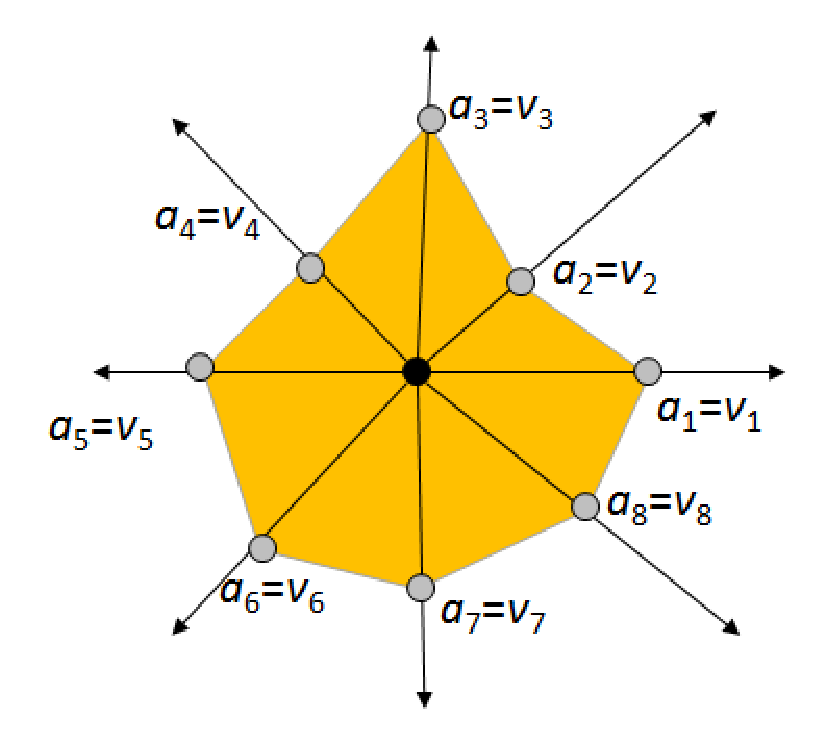
\includegraphics[width=0.5\linewidth]{images/StarplotExample.eps}
  \caption{An example of a Starplot glyph. }
	\label{fig:StarplotExample}
\end{figure}

\subsection{Supporting Comparison and Clustering}
\label{sec:ComparisonSupport}
To support analysis questions discussed in Section~\ref{sec:DOIAnalysisTasks}, DOIs must support comparisons. Gleicher et al. proposed three categories for visual analysis: juxtaposition, superposition, and explicit encoding~\cite{Glei11}. In juxtaposition, two visualization placing side by side facilitate comparison. Next, in superposition, we can render one visualization over another to aid similarity among them. Finally, in explicit encoding, we can describe explicit relationship visually by encoding two data in a single view.

Visual analyses are not limited to the above mentioned categories. Besides, the three categories are the basic categories. We can generate hybrid categories from them. In Figure~\ref{fig:ComparisonCategories}, we describe an example of two user data $User_1$ and $User_2$. Figure~\ref{fig:ComparisonCategories}(i) depicts comparison by juxtaposing them, by superpositioning them in Figure~\ref{fig:ComparisonCategories}(ii). Figure~\ref{fig:ComparisonCategories}(iii) depicts a explicit encoding of intersection between them.  
\begin{figure}[htbp]
  \centering
  \includegraphics[width=\linewidth]{images/ComparisonCategories.eps}
  \caption{An example of comparison categories by Gleicher et al.~\cite{Glei11}. i) Juxtaposition, ii)Superposition, and iii) Explicit encoding (Intersection).}
	\label{fig:ComparisonCategories}
\end{figure}

Again, clustering support will facilitate analyzers to compare visualization with less cluttering and more associativity among data. Kurzhal et al.~\cite{Kur14} described a clustering method using string-edit distance of AOI sequences. 

\subsection{Supporting Interactions}
DOI data analysis will be largely impacted by using interactive visualization and visual analytics. Kurzhal et al.~\cite{Kur14} and Blascheck et al.~\cite{Bla16} already described visual analytics for AOI data. For interaction, Yi et al.~\cite{Yi07} proposed seven categories of interaction for information visualization: encoding, comparison, selection, reconfiguration, exploration, abstract/elaborate, and filtering. We already described about encoding in Section~\ref{sec:LargeDataSupport} and Section~\ref{sec:DataAttributeSupport}, about comparison in Section~\ref{sec:ComparisonSupport}. We discuss the rest of them in context of DOI data below. 

\noindent \textbf{Selection :} Selections allow users to track interesting objects by marking them~\cite{Yi07}. With respect to selection targets, DOI methods support selections of DOIs, DOI categories, users, and time intervals.  As for methods of selection, two options are possible: `in situ' selections of DOIs shown in the visualization, and query-based selections of DOIs by attribute values. Finally, selected items should be highlighted visually and brushing and linking should translate selections over multiple views, supporting connect and compare interactions. 

\noindent \textbf{Reconfiguration :}
Reconfigurations change the spatial arrangement of data.  We already discussed the benefit of clustering co-viewed DOIs to reduce clutter and to support the detection of correlations between DOI categories and when they are viewed. Additionally, DOIs should be orderable based on their attributes. Similarly, clustering and arranging subjects by their behavior can create more organized visualizations, while the ability to cluster subjects on their background or demographic data (e.g., expert vs. naive subjects) can support tasks typical of human experimentation. Finally, visualizations should also support interactive repositioning (e.g., of users, DOIs), to allow analysts to manually arrange and group items.


\noindent \textbf{Exploration} enables users to analyze different subsets of data instances. DOI data visualizations should support time-scrolling, panning, and zooming efficiently. Exploration options also include the ability to flexibly define which DOI attributes should be mapped visually, given that the number of variables that can be visually encoded concurrent may be limited. 
	
\noindent \textbf{Abstract/Elaborate} interactions allow users to control a visualization's level of abstraction. Our discussion on encoding emphasizes the need for representations that support analyses at multiple time-scales, DOI grouping, and the ability to control the amount of data shown. 

First, semantic zooming can be an efficient way to explore different time scales and involves aggregating and summarizing data over variable time-steps (e.g., milliseconds to minutes). An alternative to semantic zooming are pixel based techniques which allow individual viewing-events to merge and blend together visually\cite{keim2000designing}. 

Second, DOIs could be grouped by using attribute queries to define DOI categories, by exploiting DOI hierarchies (i.e., DOIs that are contained by other DOIs), or manually. Aggregating DOIs visually can again be done semantically, by allowing analysts to explicitly collapse multiple DOIs into single ones, or by showing data in a way that allows categories to emerge and separate visually. 

 Finally, details on demand can give access to additional data via tool-tips and auxiliary information data panels, populated with data obtained through brushing and linking.
  
	
\noindent \textbf{Filtering} enables users to change the set of data items being presented based on specific conditions, and should be possible on all selectable data categories previously mentioned. DOIs should be hidden or revealed based on their attributes, how often they are viewed, when they are viewed, and which users view them (e.g., ``Show only DOIs that both of two selected users viewed'').
	
\section{Case Studies}
Heatmap, Scarfplot. 

\section{Evaluation}
Construction
\section{Conclusion}